%-------------------------------------------------------------------------------
%	PACKAGES
%-------------------------------------------------------------------------------
\documentclass[a4paper, 11pt, twoside]{book}
\usepackage[hmarginratio=3:2]{geometry}
\usepackage[hidelinks]{hyperref}
\usepackage[brazilian]{babel}
\usepackage[utf8x]{inputenc}
\usepackage{subcaption}
\usepackage{mdframed}
\usepackage{enumitem}
\usepackage{graphicx}
\usepackage{parskip}
\usepackage{amsmath}
\usepackage{float}
\usepackage{cb}
\usepackage{ulem}
\usepackage{listings}
\usepackage[yyyymmdd,hhmmss]{datetime}
\begin{document}
	\frontmatter
	
	%-----------------------------------------------------------------------------
	%	TITLE PAGE
	%-----------------------------------------------------------------------------
	\begin{titlepage}
		% No style in cover
		\thispagestyle{empty}
		% Centraling content in page
		\newgeometry{margin=1in}
		\center
		
		%	HEADING SECTIONS
		%\textsc{\LARGE Universidade de Brasília}\\[1.5cm] % Name of your university/college
		%\textsc{\Large Notas de Aula}\\[5cm] % Major heading such as course name
		
		%	TITLE SECTION
		\HRule \\[0.4cm]
		{\huge \bfseries Computação Básica}\\[0.4cm]
		\HRule \\[6.5cm]
		
		%	AUTHOR SECTION
		\begin{minipage}{0.4\textwidth}
			\begin{flushleft} \large
				\emph{Autor:}\\
				Guilherme \textsc{Branco} % Your name
			\end{flushleft}
		\end{minipage}
		%	DATE SECTION
		\vfill
		{\large \today}\\[2cm]
	\end{titlepage}
	
	%-----------------------------------------------------------------------------
	%	CONTENT
	%-----------------------------------------------------------------------------
	% Default margins for the rest of the document
	\restoregeometry
	
	% Index
	\tableofcontents
	
	% Content
	\mainmatter
	\chapter*{Sobre este Documento}

Este resumo tem o objetivo de auxiliar o leitor nos tópicos básicos de Computação. Este documento foi gerado em \today{} às \currenttime. Para contribuições ou acompanhamento do material, acesse o repositório oficial: \url{ainda não existe}. \\

O conteúdo não possuíra uma linguagem específica a ser seguida, as explicações serão em pseudo-código, porém algumas seções podem conter exemplos em C ou Python.

Utilize o apêndice contendo exercícios como complemento. Os exercícios geralmente ajudam a conceituar alguns pontos da matéria por outra perspectiva, mesclando algumas partes do conteúdo. Os exercícios podem ser feitos na linguagem de sua preferência.

Caso você encontre algum erro, seja conceitual, gramático ou ortográfico, envie o problema no repositório do projeto (por meio de \textit{Issue}, ajudando a contribuir para melhorar este documento.

O que ainda não esta pronto será adicionado aos poucos conforme o tempo do escritor.

TODO:
    Conteúdo em si referente a computação básica:
        -Introdução (variáveis, entrada e saída)
        -Estruturas condicionais
        -Estruturas de repetição
        -Ponteiros - Basíco (sem estrutura de dados)
        -Vetores
        -Matrizes
        -Strings
        -Funções
        -Registros (typedef, struct, para python classes simples, dicionarios ou named tuples)
        -Arquivos
        -Recursividade
    Exercícios:
        -Ponteiros - Basíco (sem estrutura de dados)
        -Vetores
        -Matrizes
        -Strings
        -Funções
        -Registros (typedef, struct, para python classes simples, dicionarios ou named tuples)
        -Arquivos
        -Recursividade

Alguns exercícios até repetição já estão escritos, previsão do conteúdo destes até o fim do carnaval.
Bons estudos!
	\chapter{Introdução}
\section{Conceitos básicos}
Existem conceitos que permeiam todas as linguagens, tais como:
\begin{itemize}
    \item Constantes e Variáveis
    \item Palavras reservadas
    \item Expressões Aritméticas
    \item Expressões Lógicas
    \item Comandos de Atribuição
    \item Entrada/Saída de dados
\end{itemize}
Esta seção tem como objetivo situar o leitor sobre estes conceitos.
\subsection{Constantes e Variáveis}
Estes dois conceitos tem em comum a alocação de uma região de memória no computador para guardar dados, porém para as constantes esse dado não pode ser modificado após sua criação, já para variáveis pode-se mudá-lo quantas vezes forem necessárias. Em ambos os casos necessita-se também do tipo de dado a ser guardado pelo computador, isto varia de linguagem, porém os tipos padrões constiuem os seguintes:
\begin{itemize}
    \item Númericos
    \begin{itemize}
        \item Inteiro - Ex.: 30, -15, 10, 0 ...
        \item Ponto Flutuante (Reais) - Ex.: 2.3, -1.2, 15.3 ...
    \end{itemize}
    \item Literais (Caracteres e Strings) - Ex.: "teste", "t", "sera" ...
    \item Lógicos (Booleano - Matemático George Boole) - Ex.: Verdadeiro e Falso
\end{itemize}
Em linguagens como C, C++ e Java há a necessidade de explicitar o tipo de dado ao se alocar a região de memória, em outras como Python ou PHP não há explicitamente o tipo ao se definir uma variável ou constante. \\
Exemplo em C e em seguida em Python:
\begin{lstlisting}
    //Comentario em C
    int a = 1;
    const int b = 2;
    float c = 2.3;
    const float d = 3.2;
    char e = 'a';
    const char f = 'b';
\end{lstlisting}
\begin{lstlisting}
    #Comentario em Python
    a = 1
    c = 2.3
    e = 'a'
\end{lstlisting}
Note que em Python não há a palavra const, não sendo possível criar constantes de verdade.
\subsection{Palavras reservadas}
Existem palavras reservadas que diferem de linguagem para linguagem, elas servem para diversas coisas, como definir um tipo de dado, declarar uma constante, dar comandos condicionais (se senão), comandos de repetição entre outros.
\subsection{Expressões Aritméticas}
Servem para fazer os cálculos utilizados no programa, os operadores mais comuns são: +, - , / , *.\\ 
Exemplo: $ a + b $
\subsection{Expressões Lógicas}
Fazer cálculos booleanos, que resultem em Verdadeiro ou Falso, os operadores mais comuns são: \&\& (E) e || (OU), existindo também os de maior que e menor que e outros. E seus reultados seguem a tabela verdade, como em \ref{tab:vE} e \ref{tab:vOU}.
Exemplo: \\
\begin{table}[!h]
\centering
\caption{Tabela verdade para operador E}
\label{tab:vE}
\begin{tabular}{llll} \hline \hline
0 & 1 &  &  \\
&   &  &  \\
&   &  &  \\ \hline \hline
\end{tabular}
\end{table}

\begin{table}[!h]
\centering
\caption{Tabela verdade para operador OU}
\label{tab:vOU}
\begin{tabular}{lll}
OU & F & V \\
F  & F & V \\
V  & V & V
\end{tabular}
\end{table}
\subsection{Comando de Atribuição}
Para atribuir um valor a uma variável tem-se o comando de atribuição, na maioria das linguagens se utiliza o comando '=' para tal. \\
Exemplo: $ a = 2 $ \\
Porém, algumas linguagens podem utilizar a sequência ``:='' entre outros.
\subsection{Entrada e Saída}
O computador esta configurado para ter uma saída padrão, o monitor, e uma entrada padrão, o teclado. Para acessar as estas funcionalidades, existem meios de requisitar a entrada de dados do usuário ou de mostrar algo na tela. Por didática será utilizado:
\begin{itemize}
    \item Print(<palavra>) - Para escrever na tela
    \item Input(<variavel>) - Para ler do teclado o que foi digitado
\end{itemize}
Mas vale lembrar que nas linguagens isto pode não estar desta forma, variando o comando para cada linguagem. Em C, por exemplo, o comando parar ler do teclado constitui o ``scanf()'' já para mostrar na tela o ``printf()''.

\section{Algoritmos}
Agora que sabemos alguns comandos de linguagens de programação podemos construir algoritmos simples, para tal devemos definir o que será o algoritmo: \\
\begin{definicao}{Algoritmo}
    Um algortimo constitui uma sequência de passos finita, com instruções bem definidas e não ambíguas.
\end{definicao}

Vamos montar agora um problema para resolver a transformação de graus Celsius para Fahrenheit:
\begin{equation}
    T_{F} = T_{C} * \frac{9}{5} + 32
\end{equation}

\begin{lstlisting}
    real celsius, fahrenheit;
    Input(celsius)
    fahrenheit = celsius * (9/5) + 32
    Escreva(fahrenheit)
\end{lstlisting}
	\chapter{Estruturas Condicionais}
\section{Condições}
Em alguns algoritmos, como os vistos no capítulo anterior, a execução se dá de maneira pré-definida, porém estruturas condicionais servem para modificar o fluxo do algoritmo, como decidir se deve ser utilizado o bloco de instruções A ou B, vide Figura \ref{fig:fluxo}.
\begin{figure}[!h]
    \centering
    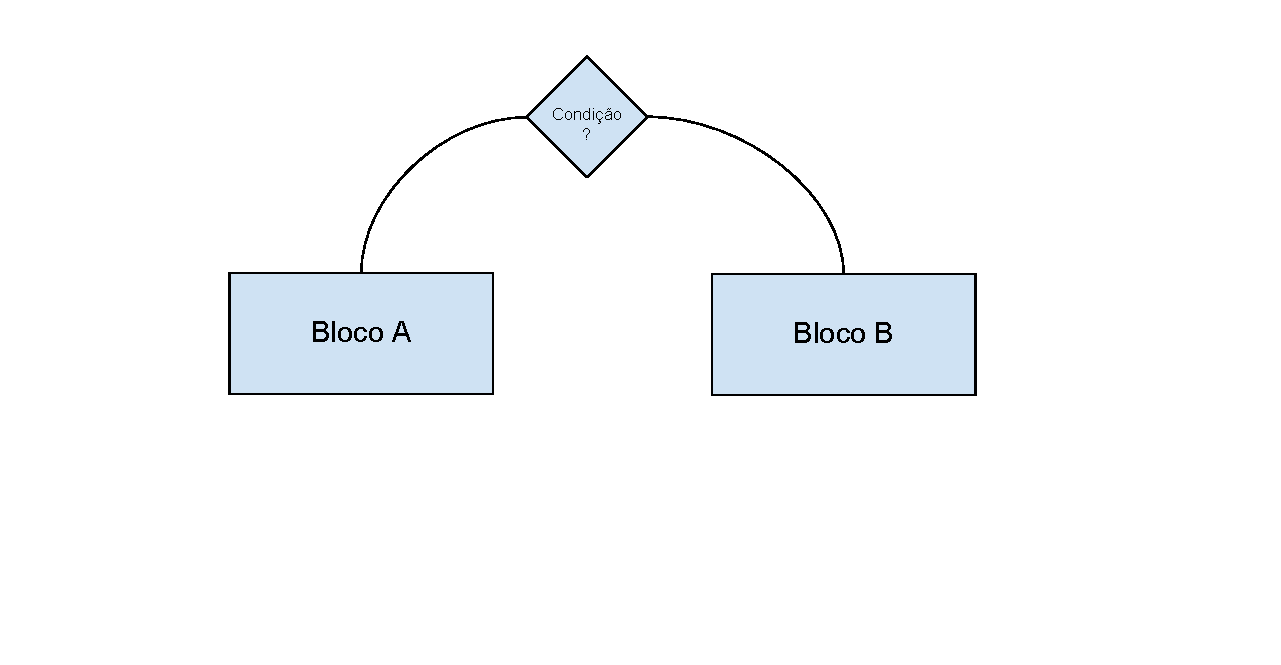
\includegraphics[scale=.5]{condicional.pdf}
    \caption{Fluxograma condicional}
    \label{fig:fluxo}
\end{figure}
Basicamente uma pergunta que deve ser respondida com os tipos lógicos Verdadeiro ou Falso, e pode ser utilizado em conjunto com os operadores lógicos, alguns presentes na tabela \ref{tab:operadoresLogicos}.
\begin{table}[!h]
\centering
\caption{Operadores lógicos}
\label{tab:operadoresLogicos}
\begin{tabular}{cc} \hline \hline
Operador      & Definição          \\ \hline
\&\&          & E                  \\
||            & OU                 \\
\textgreater  & Maior que          \\
\textgreater= & Maior ou igual que \\
\textless     & Menor que          \\
\textless=    & Menor ou igual que \\ \hline \hline

\end{tabular}
\end{table}

As estruturas condiconais podem ser simples ou compostas, a seguir têm-se o funcionamento das duas estruturas, começando pela simples.
\begin{lstlisting}
    Se <condicao> entao
        <comando1>
        <comando2>
        .
        .
        .
        <comandoN>
    Fim-Se
\end{lstlisting}
\textbf{Exemplo:} \textbf{Se} um cliente queira que suas compras sejam embrulhadas para presente deverá pagar uma taxa adicional de R\$$3,50$. Logo, para calcular o preço total deve-se saber se a mercadoria deve ser embrulhada.
\begin{lstlisting}
    valor: real
    presente: caracter
    Escreva("Informe o valor da mercadoria: ")
    Leia(valor)
    Escreva("Deseja embrulhar para presente?")
    Leia(presente)
    Se presente == 'S' entao
        valor = valor + 3.5
    Fim-Se
    Escreva("Total a pagar : " + valor)
\end{lstlisting}
Note que caso a informação guardada na variável presente for equivalente ao caracter 'S' então o valor da compra terá um acréscimo referente ao valor do embrulho. \\
Para as estruturas compostas temos a adição de duas novas palavras reservadas: o senão e o senão-se. Que servem para o caso contrário da condição, ou para condições extras, por exemplo: \\
Dados três números distintos, elabore um algoritmo que escreva o maior número digitado.
\begin{lstlisting}
    a,b,c: inteiro
    Leia(a, b, c)
    Se (A>B) entao
        Se (A>C) entao
            Escreva("O maior numero e A")
        Fim-Se
    Senao
        Se (B>C) entao
            Escreva("O maior numero e B")
        Senao
            Escreva("O maior numero e C")
        Fim-se
    Fim-Se
\end{lstlisting}
Note que o senão não precisa de condição, pois utiliza o contrário da condição do Se anterior. Podemos melhorar o algoritmo acima utilizando o senão se:
\begin{lstlisting}
    a,b,c: inteiro
    Leia(a, b, c)
    Se (A>B) E (A>C) entao
        Escreva("O maior numero e A")
    Senao Se (B>C) entao
        Escreva("O maior numero e B")
    Senao
        Escreva("O maior numero e C")
    Fim-Se
\end{lstlisting}
Isto funciona pois utiliza-se o operador lógico E na condição, logo se A>B e A>C, o A é o maior. Porém se falhar na condição de A>B, temos de testar B>C para decidir qual dos outros será o maior. Note também que podemos fazer estrutras condicionais equivalentes utilizando o operador lógico da negação (!).
\begin{lstlisting}
    Se <condicao> entao
        <comandos1>
    Senao
        <comandos2>
    Fim-se
\end{lstlisting}
\begin{lstlisting}
    Se !<condicao> entao
        <comandos2>
    Senao
        <comandos1>
    Fim-se
\end{lstlisting}
As duas estruturas se tornam equivalentes, pois inverte-se a ordem em que os comandos serão dados, na primeira estrutura os comandos1 vão ser executados, já na segunda os comandos2.
	\chapter{Estruturas de repetição}
Essas estruturas servem para, como o nome já implica, repetir um trecho do algoritmo, seja para garantir que a entrada de dados esteja correta, para refazer uma ação $n$ vezes ou para manter o algoritmo em funcionamento por tempo indeterminado (como no caso de um jogo, onde o jogo só termina quando o usuário pede para sair). Existem três tipos de comandos para repetição, Para, Enquanto e Faça-Enquanto, que são equivalentes entre si, ou seja, pode ser utilizado o de sua preferência.
\section{Contadas}
A repetição contada pode ser utilizada quando sabe-se a quantidade de vezes que o laço deverá ocorrer. Esta quantidade pode ser informada pelo usuário ao se atribuir o valor para uma variável. O comando mais comum para a repetição contada constitui o ``Para''\\
\begin{lstlisting}
    Para <variavel> = <valor_inicial> ate <condicao> em passos de <incremento> faca
        <comandos>
        .
        .
        .
    Fim-Para
\end{lstlisting}
Exemplo: Determine a média aritmética de $n$ números.
\begin{lstlisting}
    n, i: inteiro
    soma, nro: real
    Leia(n)
    Soma = 0
    Para i=0 ate i<n em passos de i=i+1 faca
        Leia(nro)
        soma = soma + nro
    Fim-Para
    Escreva(soma/n)
\end{lstlisting}
Note que de $i = 0$ até $i < n$ existem $n$ repetições de 1 em 1. Por exemplo, de $0$ a $5$ passamos pelos números, $0$, $1$, $2$, $3$ e $4$, totalizando $5$ números.
\section{Repetições com teste no começo}
O teste no começo serve para checar se o bloco de código deve ser executado ou se deve ser pulado. Pode ser utilizado com a estrutura anterior (Para ... até ... em passos de ...), porém mais comumente utilizado com uma nova estrutura, o Enquanto: \\
\begin{lstlisting}
    <variavel> = <valor_inicial>
    Enquanto <condicao> faca
        <incremento>
        <comandos>
    Fim-Enquanto
\end{lstlisting}
Note que nesta estrutura deve-se inicializar a variável fora do comando da repetição, assim como o incremento fica entre os comandos do bloco e não na repetição em si. Vamos montar o algoritmo para calcular $n!$ (fatorial). \\
Ideia do algoritmo:
\begin{lstlisting}
    Decalaracao de variaveis
    Leia(n)
    Calcula(n!)
    Mostra(n!)
\end{lstlisting}
Já se sabe como declarar, ler e mostrar valores, o calculo de n! se dará por repetição:
\begin{lstlisting}
    fat = 1
    i = 2
    Enquanto (i <= n) faca
        fat = fat*i
        i = i+1
    FimEnquanto
\end{lstlisting}
Para garantir o funcionamento pode-se utilizar o teste de mesa na Tabela \ref{tab:testefatorial}, começando com $n = 5$, por exemplo:
\begin{table}[!h]
    \centering
    \caption{Teste de mesa para o fatorial de 5}
    \label{tab:testefatorial}
    \begin{tabular}{ccccc} \hline \hline
    n & i & (i\textless=n) & fat & saida               \\ \hline
    5 & 2 & Sim            & 2   &                     \\
    5 & 3 & Sim            & 6   &                     \\
    5 & 4 & Sim            & 24  &                     \\
    5 & 5 & Sim            & 120 &                     \\
    5 & 6 & Nao            & -   & Fatorial de 5 é 120 \\ \hline \hline
    \end{tabular}
    \end{table}
\section{Repetições com teste no fim}
Esta última estrutura serve para checar se o bloco de código deve continuar a ser executado, portanto, sempre rodará pelo menos uma vez, já que o teste só aparece ao fim do bloco.
\begin{lstlisting}
    <variavel> = <valor_inicial>
    Faca
        <incremento>
        <comandos>
    Enquanto <condicao>
\end{lstlisting}
Da mesma forma que o anterior o incremento deve ser colocado junto aos comandos do bloco. Para exemplo será feito um algoritmo que calcula a soma de valores até que um valor negativo seja lido.
\begin{lstlisting}
    valor: inteiro
    soma: inteiro
    soma = 0
    Faca
        Escreva("Informe um numero")
        Leia(valor)
        soma = soma + valor
    Enquanto (valor >= 0)
    Escreva(soma)
\end{lstlisting}
Para desconsiderar o valor negativo da soma deve-se subtrai-lo ao final da repetição ou adicionar uma condição para não soma-lo durante os comandos da repetição.
\begin{lstlisting}
    valor: inteiro
    soma: inteiro
    soma = 0
    Faca
        Escreva("Informe um numero")
        Leia(valor)
        soma = soma + valor
    Enquanto (valor >= 0)
    soma = soma - valor
    Escreva(soma)
\end{lstlisting}
ou
\begin{lstlisting}
    valor: inteiro
    soma: inteiro
    soma = 0
    Faca
        Escreva("Informe um numero")
        Leia(valor)
        Se (valor >= 0)
            soma = soma + valor
        Fim-Se
    Enquanto (valor >= 0)
    Escreva(soma)
\end{lstlisting}
	\chapter{Vetores}
Com os conhecimentos até o momento caso seja necessário mais de uma variável que faça a mesma função deve-se declarar cada uma delas separadamente, porém há uma maneira de guardar estas variáveis em posições sequenciais de memória como mostra a Figura \ref{fig:memVetor}.
\begin{figure}[!h]
    \centering
    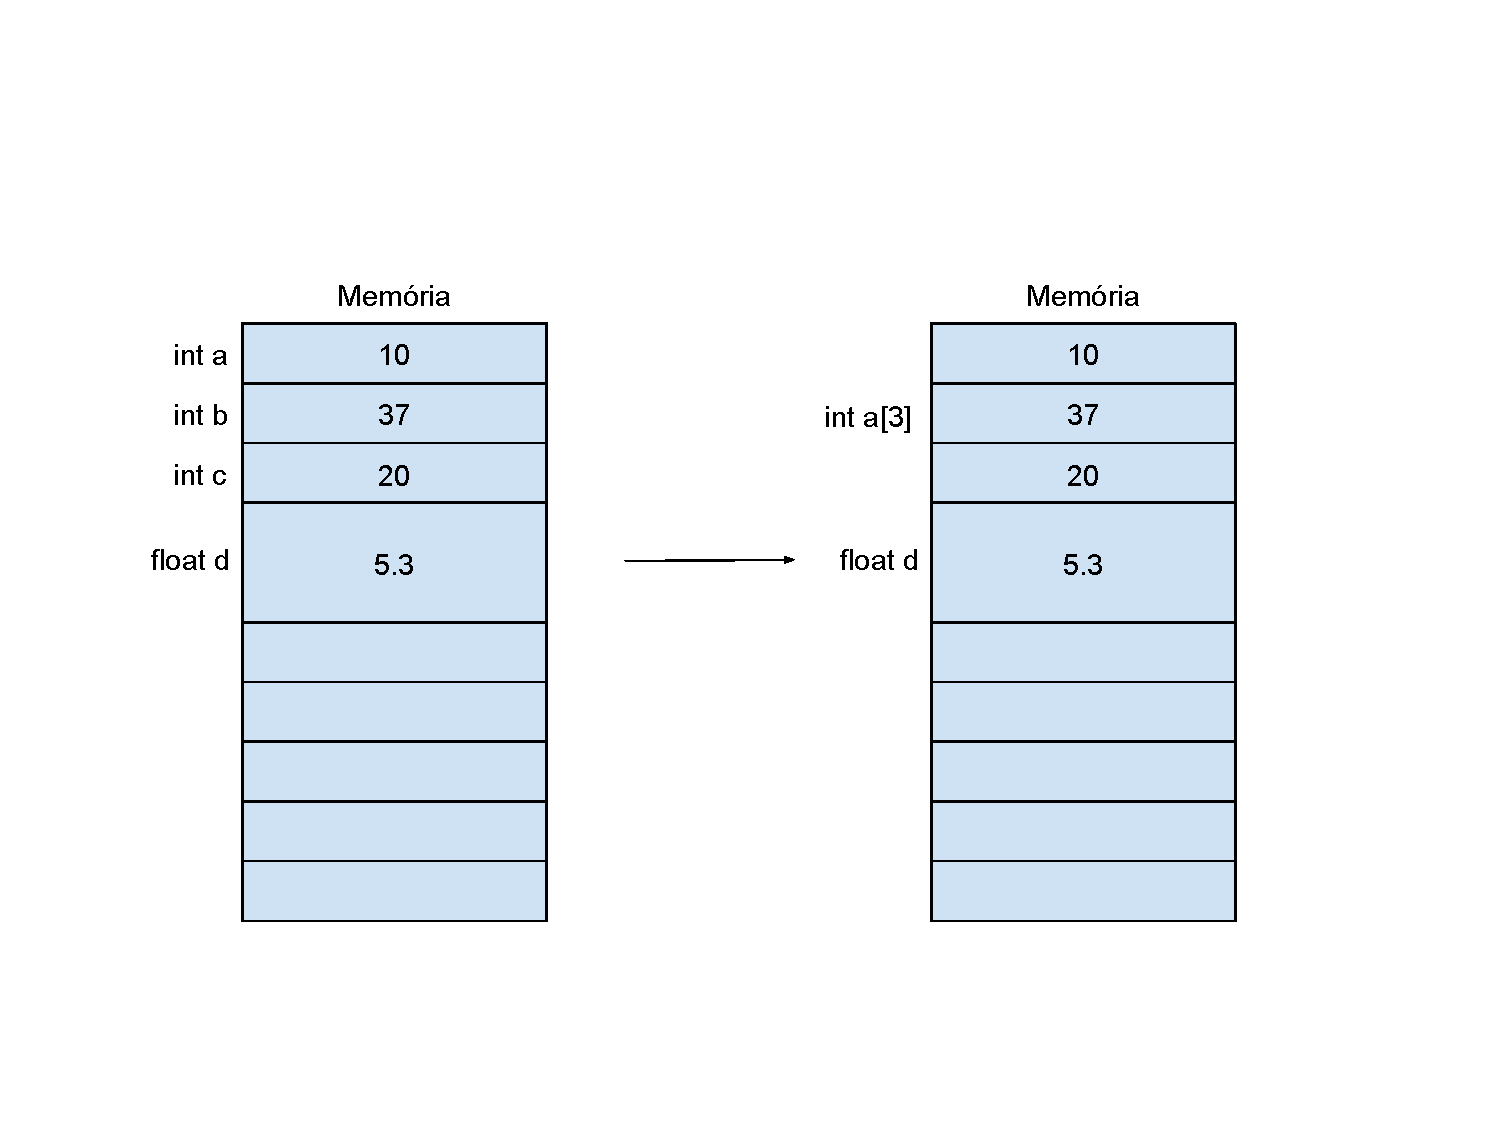
\includegraphics[scale=.5]{memVetor.pdf}
    \caption{Alocação de memória para vetores}
    \label{fig:memVetor}
\end{figure}
Desta forma o acesso as variáveis em vetor, considerando o exemplo da figura se dá por a[0] para o primeiro, a[1] para o segundo e a[2] para o terceiro, totalizando três variáveis inteiras. Considere agora que nestas três posições estejam o salário de funcionários de uma empresa e que eles receberam um aumento de 10\%, previamente precisaria-se de algo do tipo:
\begin{lstlisting}
    salario0,salario1,salario2,...,salarioN: inteiro
    Leia(salario0,salario1,salario2,...,salarioN)
    salario0 = salario0 * 1.1
    salario1 = salario1 * 1.1
    salario2 = salario2 * 1.1
    .
    .
    .
    salarioN = salarioN * 1.1
\end{lstlisting}
Note que precisaria-se de $N$ linhas para $N$ funcionários, portanto o código ficaria bem extenso, porém, pode-se utilizar uma estrutura de repetição junto de um vetor para facilitar o trabalho:
\begin{lstlisting}
    N: inteiro
    N = 10
    salario: vetor [N] de inteiro
    #Le os salarios de cada funcionario
    Para i = 0 ate N em passos de 1 faca
        Leia(Salario[i])
    Fim-Para
    #Calcula os 10% de aumento
    Para i = 0 ate N em passos de 1 faca
        salario[i] = salario[i] * 1.1
    Fim-Para
\end{lstlisting}
Pode-se reduzir o trabalho de digitar todas as linhas para cada salário consideravelmente, desta forma os vetores provêem uma maneira mais concisa de organizar o algoritmo e as variáveis.
	\nocite{*}
	\appendix
	\chapter{Exercícios}

%
%\begin{exercicio}
%  {}
%  {}
%\end{exercicio}


\section{Introdução}
\begin{exercicio}
  {1}
  {Crie um programa que leia e imprima o seu nome, o seu endereço, e a sua idade. O programa deve imprimir mensagens solicitando que o usuário informe os dados.}
\end{exercicio}

\begin{exercicio}
  {2}
  {Faça um programa que leia dois números inteiros, $a$ e $b$, troque o conteúdo desses números e mostre os novos valores de $a$ e $b$}
\end{exercicio}

\begin{exercicio}
  {3}
  {Crie um programa que leia dois números inteiros, calcule e mostre a média aritmética entre eles.}
\end{exercicio}

\begin{exercicio}
  {4}
  {Faça um programa que calcule o volume de um cilindro circular, dados os raio e altura do mesmo. (Obs: $V = \pi * r^2 * h$, onde $\pi=3.14$, r consiste no raio e h a altura)}
\end{exercicio}

\begin{exercicio}
  {5}
  {Crie um programa que leia três coeficientes de uma equação do segundo grau $y=a*x^2 + b*x + c = 0$ e imprima o valor das raízes. Assumir que o valor do discriminante (delta) sempre será maior ou igual a zero. \\
  Teste o programa com os seguintes conjuntos: \\
  \begin{itemize}
    \item $a = 1, b = -8, c = 15, resp: x_{1} = 5 x_{2} = 3$
    \item $a = 1, b = -8, c = 0, resp: x_{1} = 8 x_{2} = 0$
    \item $a = 2, b = -6, c = 4, resp: x_{1} = 2 x_{2} = 1$
    \item $a = 4, b = 8, c = 3, resp: x_{1} = -0.5 x_{2} = -1.5$
  \end{itemize}}
\end{exercicio}

\begin{exercicio}
  {6}
  {Crie um programa para imprimir a hipotenusa de um triângulo retângulo, dados os valores dos catetos. Calcula-se a hipotenusa como a raiz quadrada da soma dos quadrados dos catetos. \\
  Teste o programa com os seguintes conjuntos: \\
  \begin{itemize}
    \item $c_{1} = 3 c_{2} = 4, resp: h = 5$
    \item $c_{1} = 12c _{2} = 9, resp: h = 15$
  \end{itemize}}
\end{exercicio}

\begin{exercicio}
  {7}
  {Faça um programa que leia as três notas de um aluno, com seus respectivos pesos. Calcule e mostre a média final deste aluno.}
\end{exercicio}

\section{Estruturas Condicionais}

\begin{exercicio}
  {1}
  {Faça um algoritmo que receba um número inteiro e verifique se esse é par ou ímpar.}
  Obs: Para decidir se um número é par ou impar basta checar se o resto de uma divisão por 2 é 0.
\end{exercicio}

\begin{exercicio}
  {2}
  {Faça um algoritmo que leia dois números inteiros e imprima uma mensagem indicando se os dois números são iguais, ou imprima o maior entre eles se forem diferentes.}
\end{exercicio}

\begin{exercicio}
  {3}
  {Faça um algoritmo que solicite a idade de uma pessoa e informe:
  \begin{itemize}
    \item Se é menor de idade
    \item Se é maior de idade e tem menos de 65 anos
    \item Se tem pelo menos 65 anos
  \end{itemize}}
\end{exercicio}

\begin{exercicio}
  {4}
  Faça um algoritmo que leia três números inteiros diferentes e os imprima na tela em ordem \textbf{crescente}.
\end{exercicio}

\begin{exercicio}
  {5}
  {Faça um algoritmo que leia a data de nascimento de uma pessoa, dia, mês e ano, todos inteiros. Verifique se a data pode existir e imprima uma mensagem ao usuário indicando se a data está correta ou incorreta.}
  Exemplo: \\
  31/02/2003 - Fevereiro não pode ter 31
  Obs: Desconsidere anos bissextos, fevereiro sempre terá 28 dias
\end{exercicio}

\begin{exercicio}
  {6}
  {Crie um programa que leia três coeficientes de uma equação do segundo grau $y=a*x^2 + b*x + c = 0$ e imprima o valor das raízes. Calcule as raízes se o valor do discriminante (delta) for maior ou igual a zero. Se for menor que zero, apenas imprima uma mensagem adequada e interrompa o programa. \\
  Teste o programa com os seguintes conjuntos: \\
  \begin{itemize}
    \item $a = 1, b = -8, c = 15, resp: x_{1} = 5 x_{2} = 3$
    \item $a = 1, b = -8, c = 0, resp: x_{1} = 8 x_{2} = 0$
    \item $a = 2, b = -6, c = 4, resp: x_{1} = 2 x_{2} = 1$
    \item $a = 4, b = 8, c = 3, resp: x_{1} = -0.5 x_{2} = -1.5$
    \item $a = 4, b = 2, c = 1, resp: discriminante menor que zero$
  \end{itemize}}
\end{exercicio}

\begin{exercicio}
  {7}
  {Dado um número inteiro, permitir ao usuário escolher dentre uma lista (menu) qual operação o mesmo deseja realizar: \\
  \begin{itemize}
    \item verificar se o número é par
    \item verificar se é ímpar
    \item verificar se é múltiplo de 3
    \item verificar se é múltiplo de 5
    \item verificar se é múltiplo de 7
    \item verificar TODOS os testes
  \end{itemize}}
\end{exercicio}

\begin{exercicio}
  {8}
  {O Departamento do Meio Ambiente mantém três listas (A, B e C) de indústrias conhecidas por serem altamente poluentes da atmosfera. Os resultados de várias medidas são combinados para formar o que é chamado de "índice de poluição". Isto é controlado regularmente. Normalmente os valores caem entre $0.05$ e $0.25$. Se o índice de poluição atingir $0.25$ a situação é de alerta; se atingir $0.3$, as indústrias da lista A serão chamadas a suspender as operações até que os valores retornem ao normal. Se atingir $0.4$, as indústrias B serão também notificadas. Se exceder $0.5$, as três serão avisadas. \\
  Escreva um programa para ler o índice de poluição e emitir um relatório notificando as indústrias, caso necessário. Deve constar no relatório a situação ocorrida (abaixo, normal ou alerta). \\
  Teste o programa com os seguintes conjuntos: \\
  \begin{itemize}
    \item $i = 0.26, resp: Alerta$
    \item $i = 0.03, resp: Abaixo do normal$
    \item $i = 0.3, resp: Lista A suspensa$
    \item $i = 0.06, resp: Normal$
    \item $i = 0.4, resp: Listas A e B suspensas$
    \item $i = 0.35, resp: Lista A suspensa$
    \item $i = 0.53, resp: Listas A, B e C suspensas$
  \end{itemize}}
\end{exercicio}

\begin{exercicio}
  {9}
  {Dado três valores de um suposto triângulo, decidir se esses valores podem ou não ser um triângulo, e cao seja decidir se é um triângulo retângulo ou não. \\
  Dado que: \\
  \begin{itemize}
    \item Para ser triângulo a soma de dois lados sempre tem que ser maior que outro
    \item Para ser triângulo retângulo o maior lado ao quadrado tem que ser igual a soma dos quadrados dos outros dois
  \end{itemize}}
\end{exercicio}

\begin{exercicio}
  {10}
  {Dado o ponto de origem (x,y), a altura A e largura L num epsaço bidimensional, podemos definir um retângulo. Receber um ponto (a,b) e decidir se ele esta:
  \begin{itemize}
    \item Dentro
    \item Fora 
    \item Em alguma das linhas que definem o retângulo
  \end{itemize}}
\end{exercicio}

\section{Estruturas de repetição}
\subsection{Contada}
\begin{exercicio}
  {1}
  {A conversão de graus Fahrenheit para Celsius é obtido por c=(5/9)*(f-32). \\
  Faça um algoritmo que calcule e escreva uma tabela de garus Fahrenheit e graus Celsius, cujos graus variem de 50 a 65, de 1 em 1.}
\end{exercicio}
\begin{exercicio}
  {2}
  {Faça um algortimo que apresente a soma acumulada de todos os valores entre 1 e 100.}
\end{exercicio}
\begin{exercicio}
  {3}
  {Faça um algoritmo que leia dez números que representam notas de dez alunos, obtenha:
  \begin{itemize}
    \item A soma das notas
    \item A média das notas
    \item A maior nota
    \item A menor nota
  \end{itemize}}
  Obs: Assuma que todas as notas são informadas corretamente no intervalo de 0 a 10.
\end{exercicio}
\begin{exercicio}
  {4}
  {Faça um algoritmo que exiba a tabuada dos números de 10 a 20.}
\end{exercicio}
\begin{exercicio}
  {5}
  {Um funcionário de uma empresa recebe aumento salarial anualmente. \\
  Sabe-se que:
  \begin{itemize}
    \item Esse funcionário foi contratado em 1995, com salário inicial de R\$$1000$
    \item Em 1996 recebeu aumento de $1,5$\%
    \item A partir de 1997(inclusive), os aumentos sempre corresponderam ao dobro do percentual anterior
  \end{itemize}
  Faça um algoritmo que determine o salário atual desse funcionário.}
\end{exercicio}
\begin{exercicio}
  {6}
  {Faça um algoritmo que leia dez conjuntos de dois valores, o primeiro representa a matrícula do aluno e o segundo a sua altura em centímetros. Encontre o aluno mais alto e o mais baixo. Mostre a matrícula do aluno junto com suas alturas.}
\end{exercicio}
\begin{exercicio}
  {7}
  {Faça um algoritmo qu emostre todos os números pares entre 1 a 50.}
\end{exercicio}
\begin{exercicio}
  {8}
  {Faça um algoritmo que leia o número de andares de um prédio e, para cada andar, leia o número de pessoas que entraram e saíram do elevador. Se o número de pessoas, após a entrada e saída, for maior do que $15$, deve ser mostrada a mensagem ``Excesso de Passageiros. Devem sair X"'', onde $X$ corresponde ao número que excedem. Após a entrada e saída no último andar, o algoritmo deve mostrar quantas pessoas permaneceram no elevador.}
\end{exercicio}
\subsection{Teste no começo}
\begin{exercicio}
  {1}
  {Faça um algoritmo para o seguinte problema: ler um conjunto de valores correspondentes aos pontos que alunos obtiveram em um teste. Quando o valor fornecido for um número negativo não existem mais pontos para serem lidos.
  \begin{itemize}
    \item Contar e escrever quantos alunos fizeram o teste.
    \item Contar e escrever quantos alunos tiveram nota baixa (Pontos < 5)
    \item Contar e escrever quantos alunos tiveram nota alta (5 <= Pontos <= 10)
  \end{itemize}}
\end{exercicio}
\subsection{Teste no final}
\begin{exercicio}
  Desenvolva um algoritmo que calcule o valor da soma: \\
  $S = \frac{1}{1} + \frac{3}{2} + \frac{5}{3} + \frac{7}{4} + ... + \frac{99}{50}$
\end{exercicio}
\subsection{Extras - Utilize a repetição que preferir ou faça uma vez com cada para aprender}
\begin{exercicio}
  {1}
  {Imprima o valor de: \\
  $\sum\limits_{i=1}^{10} i$}
  
  Resposta: 55.
\end{exercicio}

\begin{exercicio}
  {2}
  {Imprima o valor de $n!$, sendo $n$ informado pelo usuário. \\
  Teste para os seguintes casos: \\
  \begin{itemize}
    \item $n = 0, resp: 1$
    \item $n = 1, resp: 1$
    \item $n = 2, resp: 2$
    \item $n = 3, resp: 6$
    \item $n = 5, resp: 120$
  \end{itemize}}
\end{exercicio}

\begin{exercicio}
  {3}
  {Imprima o valor da soma: \\
  $\sum\limits_{i=1}^{200} \frac{1}{i}$}
\end{exercicio}

\begin{exercicio}
  {4}
  {Partindo-se de um único casal de coelhos filhotes recém-nascidos, supondo que um casal de coelhos torne-se fértil após dois meses de vida e partir de então, produz um novo casal a cada mês e assumindo-se que os colhes nunca morrem, a quantidade de casais de coelhos após $n$ meses se dá pelo n-ésimo termo da seguinte sequência: \\
  $F_{n} = F_{n-2} + F_{n-1}, n>=2$ \\
  $F_{0} = 0  e F_{1} = 1$ \\
  Esta sequencia se chama \textit{Fibonacci}. Imprima a quantidade de casais de coelhos após $n$ meses, onde $n$ é dado pelo usuário.}
\end{exercicio}

\begin{exercicio}
  {5}
  {Calcule e imprima a média aritmética das idades de um grupo de pessoas fornecidas pelo usuário, cada idade sendo maior que zero. A entrada dos dados é finalizada quando o usuário digitar um valor igual a $0$. \\
  Teste o programa para $60,20,30,70,45,25,0$.}

  Resposta correta: $41.66$
\end{exercicio}

\begin{exercicio}
  {6}
  {Leia as seguintes informações para um número indeterminado de alunos: matrícula (inteiro), nome (string), e as notas de três provas (reais). A leitura dos dados deve terminar quando o usuário digitar $0$ para a matrícula. Esse último valor não deve ser considerado para o cálculo. Imprima, para cada aluno: matrícula, nome e média ponderada das provas, onde a primeira prova tem peso $2$, a segunda peso $4$ e a terceira peso $4$.}
\end{exercicio}

\section{Vetores}
\begin{exercicio}
  {1}
  {Escreva um algoritmo que receba dois vetores de $25$ números inteiros cada, crie um novo vetor de $50$ posições que seja o resultado da intercalação dos vetores de $25$.}
  Exemplo: vetor1 = [1,2,3,4,5], vetor2[6,7,8,9,10]. vetor\_intercalado = [1,6,2,7,3,8,4,9,5,10]
\end{exercicio}

\begin{exercicio}
  {2}
  {Faça um programa que leia um vetor com $6$ valores inteiros e imprima a quantidade de números pares e a quantidade de números ímpares.}
  Execute com os seguintes dados:
  \begin{itemize}
    \item 1 3 2 4 5 7, resp: pares = 2 ímpares = 4
    \item 1 2 3 4 5 6, resp: pares = 3 ímpares = 3
  \end{itemize}
\end{exercicio}

\begin{exercicio}
  {3}
  {Modifique o programa anterior para ler um número qualquer de valores entre $1$ e $20$, informado pelo usuário.}
  Execute coms os seguintes dados:
  \begin{itemize}
    \item 6     1 3 2 4 5 7, resp: pares = 2 ímpares = 4
    \item 7     1 2 3 4 5 6 7, resp: pares = 3 ímpares = 4
  \end{itemize}
\end{exercicio}

\begin{exercicio}
  {4}
  {Modifique o programa anterior para receber vários conjuntos de dados, sendo que o usuário deve informar o final da leitua com um valor negativo no número de valores a serem lidos.}
  Execute com os seguintes dados:
  \begin{itemize}
    \item 6   1 3 2 4 5 7, resp: pares = 2 ímpares = 4
    \item 7   1 2 3 4 5 6 7, resp: pares = 3 ímpares = 4
    \item 3   7 6 10, resp: pares = 2 ímpares  = 1
    \item -1          resp: termina o programa
  \end{itemize}
\end{exercicio}

\begin{exercicio}
  {5}
  {Faça um programa que leia $9$ valores inteiros, armazene num vetor e imprima qual destes números são menores que zero e quais as posições em que estão guardados.}
  Execute com os seguintes dados:
  \begin{itemize}
    \item 1 -3 2 5 -4 -7 8 9 -11, resp: -3 [2] \\
                                        -4 [5] \\
                                        -7 [6] \\
                                        -11 [9] 
    \item -1 30 20 -50 40 31 8 9 13, resp: -1 [1] \\
                                           -50 [4]
  \end{itemize}
  Obs: O índice para o computador começa em 0, porém para mostrar para pessoas lembre-se de acrescentar 1
\end{exercicio}

\begin{exercicio}
  {6}
  {Faça um programa que leia a temperatura média de cada mês do ano e imprima a maior e menor temperaturas do ano e em que mês ocorreram estas temperaturas. Assuma que não exista temperaturas repetidas.}
  Execute com os seguintes dados:
  25 27 26 24 22 20 18 17 30 16 26 21, resp: menor = 17 mês = 8 \\
                                             maior = 30 mês = 9
\end{exercicio}

\begin{exercicio}
  {7}
  {Faça um programa que leia um vetor e retire os valores iguais a zero. Este vetor será compactado e as posições finais devem ser preenchidas com o valor -1. O programa deve ao final escrever o vetor compactado.}
  Obs: Não mostrar as posições do vetor que foram preenchidas com o valor -1. O vetor tem tamanho 20.
  Exemplo: 1 0 2 0 3 0 4 0 5 0 6 0 7 0 8 0 9 0 10 0 \\
  Vetor compactado: 1 2 3 4 5 6 7 8 9 10 -1 -1 -1 -1 -1 -1 -1 -1 -1 -1 \\
  Vetor mostrado: 1 2 3 4 5 6 7 8 9 10
\end{exercicio}

\begin{exercicio}
  {8}
  {Faça um programa que lê os conteúdos de dois vetores X[10] e Y[10] e os mostra. Crie, a seguir, um vetor U que seja a união de X com Y, e um vetor I que seja a intersecção. Mostre o conteúdo de I e de U. Assuma que não existam elementos repetidos dentro de cada vetor.}
\end{exercicio}

\begin{exercicio}
  {9}
  {Faça um programa que leia as notas de duas provas, números reais, de 7 alunos e armazene estas em dois vetores. Crie um terceiro vetor que armazene a média aritmética das duas notas de cada aluno. Imprima as duas notas e as médias de cada aluno, onde as notas de um mesmo aluno devem ser impressas numa única linha.}
  Execute com os seguintes dados:
  7 8 5 6 4 3 9 10 7 7 8 6 9 7 \\
  Resp: aluno1 7 8 7.5 \\
        aluno2 5 6 5.5 \\
        aluno3 4 3 3.5 \\
        aluno4 9 10 9.5 \\
        aluno5 7 7 7.0 \\ 
        aluno6 8 6 7.0 \\
        aluno7 9 7 8.0
\end{exercicio}
\end{document}
